%!TEX program = Xelatex
\documentclass{article}
%\usepackage{ctex}
\usepackage{amsmath,amscd,amsbsy,amssymb,latexsym,url,bm,amsthm}
\usepackage{epsfig,graphicx,subfigure}
\usepackage{enumitem,balance,mathtools}
\usepackage{wrapfig}
\usepackage{mathrsfs, euscript}
\usepackage[usenames]{xcolor}
\usepackage{hyperref}
\usepackage{caption}
%\usepackage{subcaption}
\usepackage{float}
\usepackage{listings}
%\usepackage{enumerate}
%\usepackage{algorithm}
%\usepackage{algorithmic}
%\usepackage[vlined,ruled,commentsnumbered,linesnumbered]{algorithm2e}
\usepackage{algorithm}  
\usepackage{algorithmicx}  
\usepackage{algpseudocode}
\usepackage{geometry}
\usepackage{setspace}

\geometry{a4paper,left=2cm,right=2cm,top=2cm,bottom=2cm}

\newtheorem{theorem}{Theorem}[section]
\newtheorem{lemma}[theorem]{Lemma}
\newtheorem{proposition}[theorem]{Proposition}
\newtheorem{corollary}[theorem]{Corollary}
\newtheorem{exercise}{Exercise}[section]
\newtheorem*{solution}{Solution}

\renewcommand{\thefootnote}{\fnsymbol{footnote}}

\newcommand{\postscript}[2]
    {\setlength{\epsfxsize}{#2\hsize}
    \centerline{\epsfbox{#1}}}

\renewcommand{\baselinestretch}{1.0}

\usepackage{url}

\title{Report For CS385 Personal Project}
\author{Yanming Liu; ID: 518030910393}

\begin{document}

\maketitle
\noindent\textbf{Declare} \\
All the code in this project is written by myself, and you can check it : \url{https://github.com/lym01803/CS385_Project1}, which is 
my personal repository. I only use third-party libraries for the following: 
\begin{itemize}
    \item Visualization, e.g. PCA, t-SNE, draw curve and histogram.
    \item SVM.
    \item HOG feature.
    \item For CNN model. The network is built by myself. But I use API for network layers, e.g. Conv, BN.
    \item Basic matrix operations. For simple models, I only use pytorch to do simple matrix operations on cuda. I do not use any advanced API, such as 
    built-in network layers, optimizers and auto-gradient. In fact, to confirm it, I set the requires\_grad attribute of tensors to False.
\end{itemize}
\textbf{Note}\\
During the project, I discussed and exchanged opinions with my classmates many times. In the analysis of logistic regression model, my opinion may 
be similar to that of my classmate Yuxuan Xiong. Please note that if there are some similarities in our analysis, it is the result of our discussion, not plagiarism.

\section{Introduction}
In this project, I do the following things:
\begin{itemize}
    \item Processed the data set;
    \item Implement several basic models: Logistic Regression, LDA, kernel based Logistic Regression, SVM and CNN;
    \item Try two regular terms: Ridge and Lasso;
    \item Visualization: HOG feature, CNN feature and distribution of LDA and Logistic Regression;
    \item Analysis: mainly about the logistic regression. 
\end{itemize}

In fact, the models in this project are all discriminative models, and they are all closely related to logistic regression: LDA and logistic regression have different goals, but they take the same way to solve 
the discrimination problem: learning a projection direction to separate data; The motivation of the SVM model comes from the discussion of the margin in linear binary discrimination problem; The kernel is an extension 
of the linear model to the nonlinear model, which is equivalent to a linear model for high-dimensional (probably non-linear) features $\phi(X)$; CNN can be regarded as using a learnable deep network to produce the features 
of input images instead of using the manual designed HOG features, which is essentially a binary classifier (logistic regression) or a multi-classifier (extension of logistic regression, sigmoid -> softmax) of the CNN based features. 
Therefore, in the subsequent analysis of the project, the discussion will mainly focus on a basic point, the linear logistic regression model. 

\section{Data Process}
\subsection{Crop and Padding}
The given data set has two format: 1. original images with character level bounding boxes; 2. The cropped images. 

Since the borders of digits are usually not square, the square cropped images mostly contain part of other digits. Although someone says 
that such noise does not affect the performance of the classifier (most likely because the translation invariance of HOG is not good), I still do not plan to use it. 

Therefore, I crop the original images by myself according to the given digit boxes, then padding the images into squares symmetrically, and then resize them to a size of $32\times 32$.
For the color to padding, I choose the average color of the border pixels of cropped images (averaged for each channel). I am not sure if such an operation meets the specifications of the CV field, 
but at least the images obtained in this way seems to be of high quality to my eyes and is suitable for training discriminative models, I think.

The comparison between the two official offered data and the data processed by myself is shown in the followed Fig. \ref{datasetimage}.

\begin{figure}[H]
    \centering
    \begin{minipage}{0.32\textwidth}
        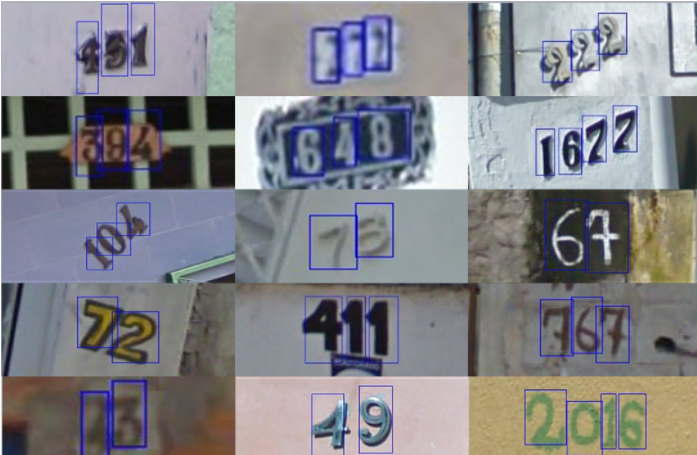
\includegraphics[width=0.95\textwidth]{fig/1.png}
        Format 1: original images
    \end{minipage}
    \begin{minipage}{0.32\textwidth}
        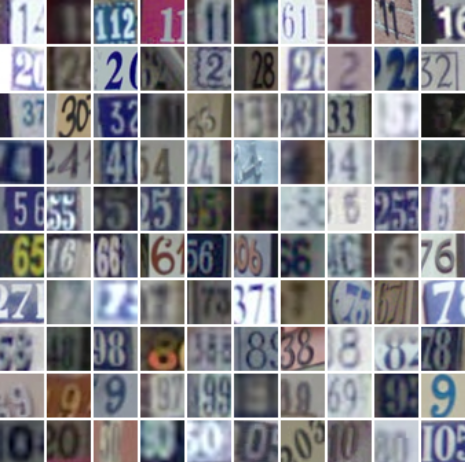
\includegraphics[width=0.95\textwidth]{fig/2.png}
        Format 2: cropped images
    \end{minipage}
    \begin{minipage}{0.32\textwidth}
        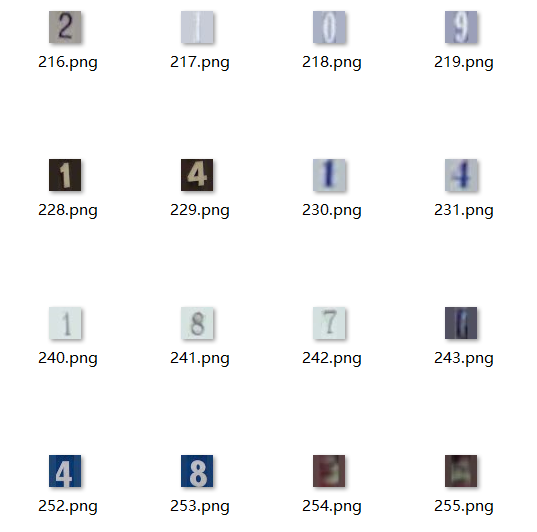
\includegraphics[width=0.95\textwidth]{fig/3.png}
        Images cropped and paddinged by myself
    \end{minipage}
    \caption{Comparison between official data and data processed by myself}
    \label{datasetimage}
\end{figure}
\subsection{HOG Feature}
General experience tells us that directly using the three-channel pixels of an image as the input features may not be effective. It is usually believed that the local gradient (both norm and direction) of an image can 
reflect image features such as object edges and textures. Therefore, the HOG feature of the image is used as the input of models (except CNN) here. A third-party library cv2.HOGDescriptor is used here. The parameters are 
shown in the following Table \ref{hogparam}, and finally $1764$-dimensional feature vectors are obtained.
\begin{table}[H]
    \centering
    \caption{The HOG parameters setting}
    \label{hogparam}
    \begin{tabular}{|lr|lr|}
        \hline
        input size& $32\times 32\times 3$&window size&$32\times 32$\\
        block size& $8\times 8$&block stride& $4\times 4$\\
        cell size & $4\times 4$& bin & 9\\
        \hline
    \end{tabular}
\end{table}

\section{Logistic Regression}
\subsection{Implement}
I follow eq. \ref{eq1}.
\begin{spacing}{1.5}
\begin{equation}
    \begin{array}{ll}
        L_i &= y_i\log p_i + (1-y_i)\log (1-p_i)\\
            &= y_iX_i^\top \beta - \log(1+\exp(X_i^\top \beta))\\
        \dfrac{\partial}{\partial\beta}L_i &= 
        y_iX_i - \dfrac{\exp(X_i^\top\beta)}{1+\exp(X_i^\top\beta)}\cdot X_i\\
            &= (y_i - p_i)\cdot X_i
    \end{array}
    \label{eq1}
\end{equation}
\end{spacing}
For efficient calculation, I do not calculate the loss $L_i$ in the program. Instead I directly calculate the gradient $\partial L_i/\partial\beta$ and perform gradient descent.  
\end{document}
